\section{Рабочий проект}
\subsection{Классы, используемые при разработке сайта}

Можно выделить следующий список классов и их методов, использованных при разработке системы тестирования (таблица \ref{class:table}).

\renewcommand{\arraystretch}{0.8} % уменьшение расстояний до сетки таблицы
\begin{xltabular}{\textwidth}{|X|p{2.5cm}|>{\setlength{\baselineskip}{0.7\baselineskip}}p{4.85cm}|>{\setlength{\baselineskip}{0.7\baselineskip}}p{4.85cm}|}
\caption{Описание классов системы тестирования, используемых в приложении\label{class:table}}\\
\hline \centrow \setlength{\baselineskip}{0.7\baselineskip} Название класса & \centrow \setlength{\baselineskip}{0.7\baselineskip} Модуль, к которому относится класс & \centrow Описание класса & \centrow Методы \\
\hline \centrow 1 & \centrow 2 & \centrow 3 & \centrow 4\\ \hline
\endfirsthead
\caption*{Продолжение таблицы \ref{class:table}}\\
\hline \centrow 1 & \centrow 2 & \centrow 3 & \centrow 4\\ \hline
\finishhead
Test & Модуль теста & Test – класс, характеризующий тест и имеющий методы для его прохождения . & def nextquestion(self): Делает инкремент id текущего вопроса и перемешивает его ответы, ничего не возвращает.
def print current question(self) - возвращает номер вопроса и его текст,
@staticmethod def shuffle(mas: []) - веремешивает переданный список и возвращает его
def start test(self) - запускает тест, обнуляет счёт и устанавливает id текущего вопроса, ничего не возвращает
def summarise(self) - Возвращает диагноз соответствующий результату теста\\
\hline FileProvider & Модуль для работы с файловой системой & FileProvider – Класс для работы с файлами & @staticmethod def savetestresult(testresult: TestResult): Сохраняет переданный результат теста, ничего не возвращает, @staticmethod
def getresults(): Получает результаты тестов из файла, возвращает список результатов,  @staticmethod def cleartestresults(): Удаляет все результаты тестов
\end{xltabular}
\renewcommand{\arraystretch}{1.0} % восстановление сетки

\subsection{Модульное тестирование разработанной системы тестирования}

Модульный тест для класса User из модели данных представлен на рисунке \ref{unitUser:image}.

\begin{figure}[ht]
\begin{lstlisting}[language=Python]
from django.test import TestCase
from .models import *
User = get_user_model()


class ShpoTestCases(TestCase):

    def setUp(self) -> None:
        self.user = User.objects.create(name="Gena")

    def test_2(self):

        self.assertEqual(self.user.name, 'Sad')
        print((self.user))
        print((self.user.name))
\end{lstlisting}  
\caption{Модульный тест класса User}
\label{unitUser:image}
\end{figure}

\subsection{Системное тестирование разработанной системы тестирования}

На рисунке \ref{authorisation:image} представлена авторизации в системе тестирования.
\begin{figure}[H] % H - рисунок обязательно здесь, или переносится, оставляя пустоту
\center{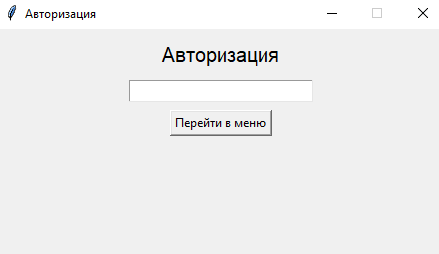
\includegraphics[width=1\linewidth]{authorisation}}
\caption{Авторизация в системе тестирования»}
\label{authorisation:image}
\end{figure}

На рисунке \ref{menu1:image} представлено меню.

\begin{figure}[H]
\center{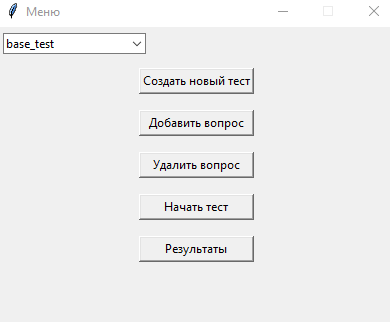
\includegraphics[width=1\linewidth]{menu1}}
\caption{Меню}
\label{menu1:image}
\end{figure}

На рисунке \ref{test:image} представлено окно теста.

\begin{figure}[H]
\center{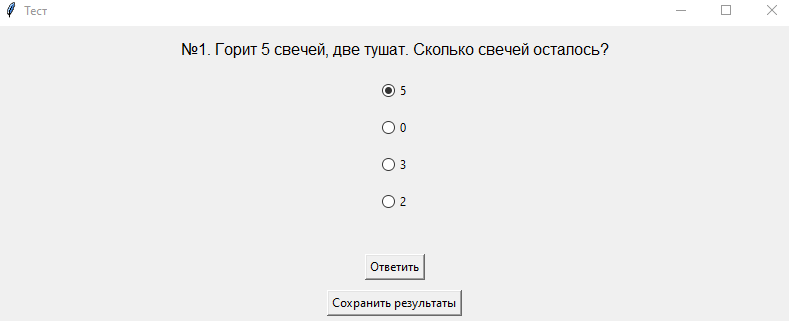
\includegraphics[width=1\linewidth]{test}}
\caption{Окно теста с одним из вопросов}
\label{test:image}
\end{figure}
